%=====================================================================
\section{Active ovals and ellipses: where the defects sit}\label{sec:sdist}
Same treatment as for circles (Sec.~\ref{sec:cdist}): time-averaged maps on a common scale and profiles against the exact distance
from the wall (Sec.~\ref{sec:m-dist}). Seed 1 of each cavity.
\begin{figure}[H]\centering
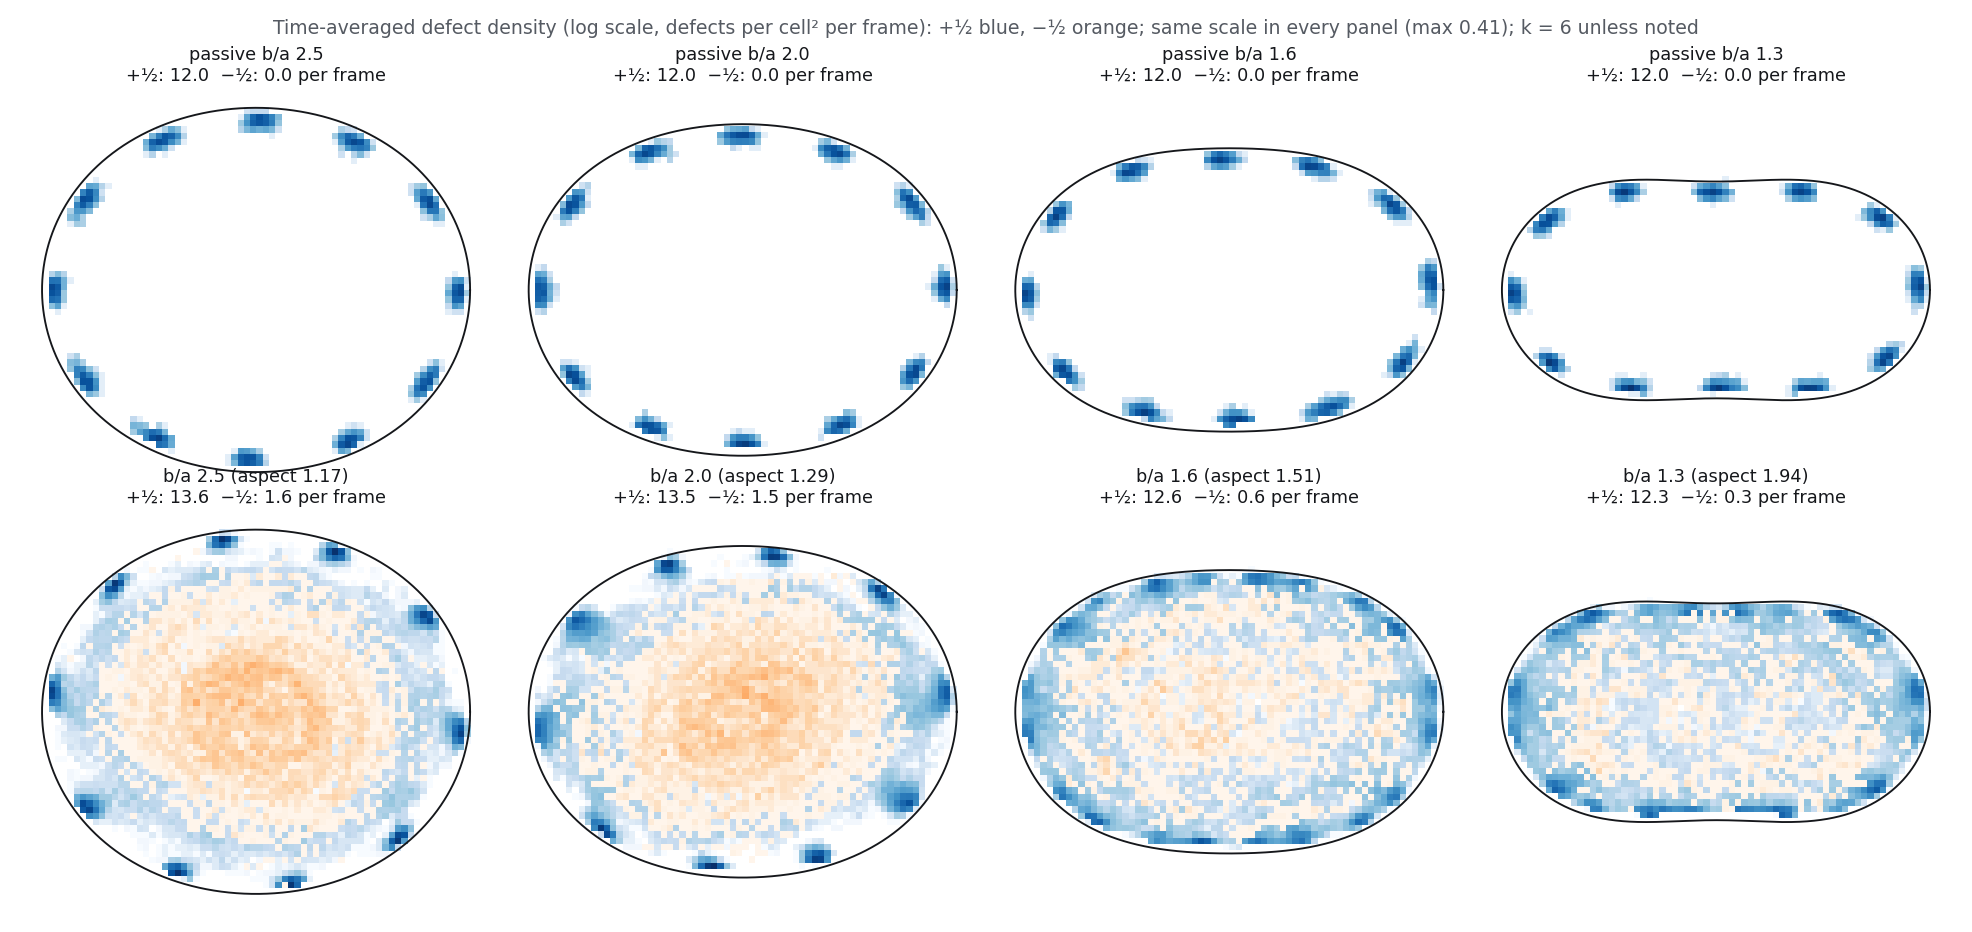
\includegraphics[width=\textwidth]{maps_ovals_small.png}
\caption{Small ovals (half-length $1.53\,\la$, the size where circles are cleanest), $k=6$: passive (top) and active (bottom),
$b/a=2.5\to1.3$ (aspect $1.17\to1.94$). Log density, common scale, $+\half$ blue, $-\half$ orange.}\label{fig:maps-small}
\end{figure}
\begin{figure}[H]\centering
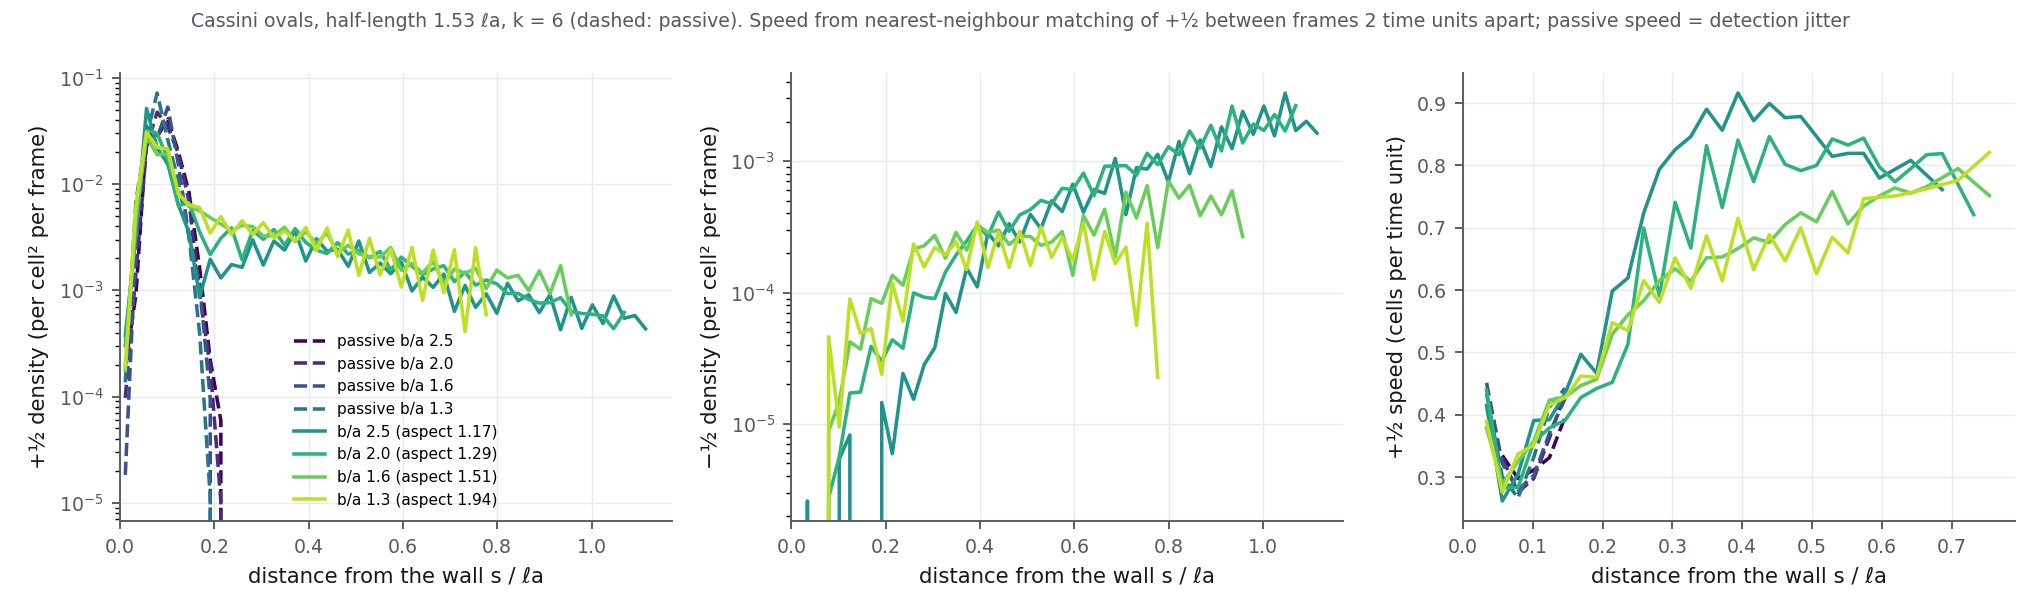
\includegraphics[width=\textwidth]{profiles_ovals_small.png}
\caption{Small ovals: $+\half$ and $-\half$ density and $+\half$ speed against the distance from the wall (dashed: passive).}\label{fig:prof-small}
\end{figure}
\begin{figure}[H]\centering
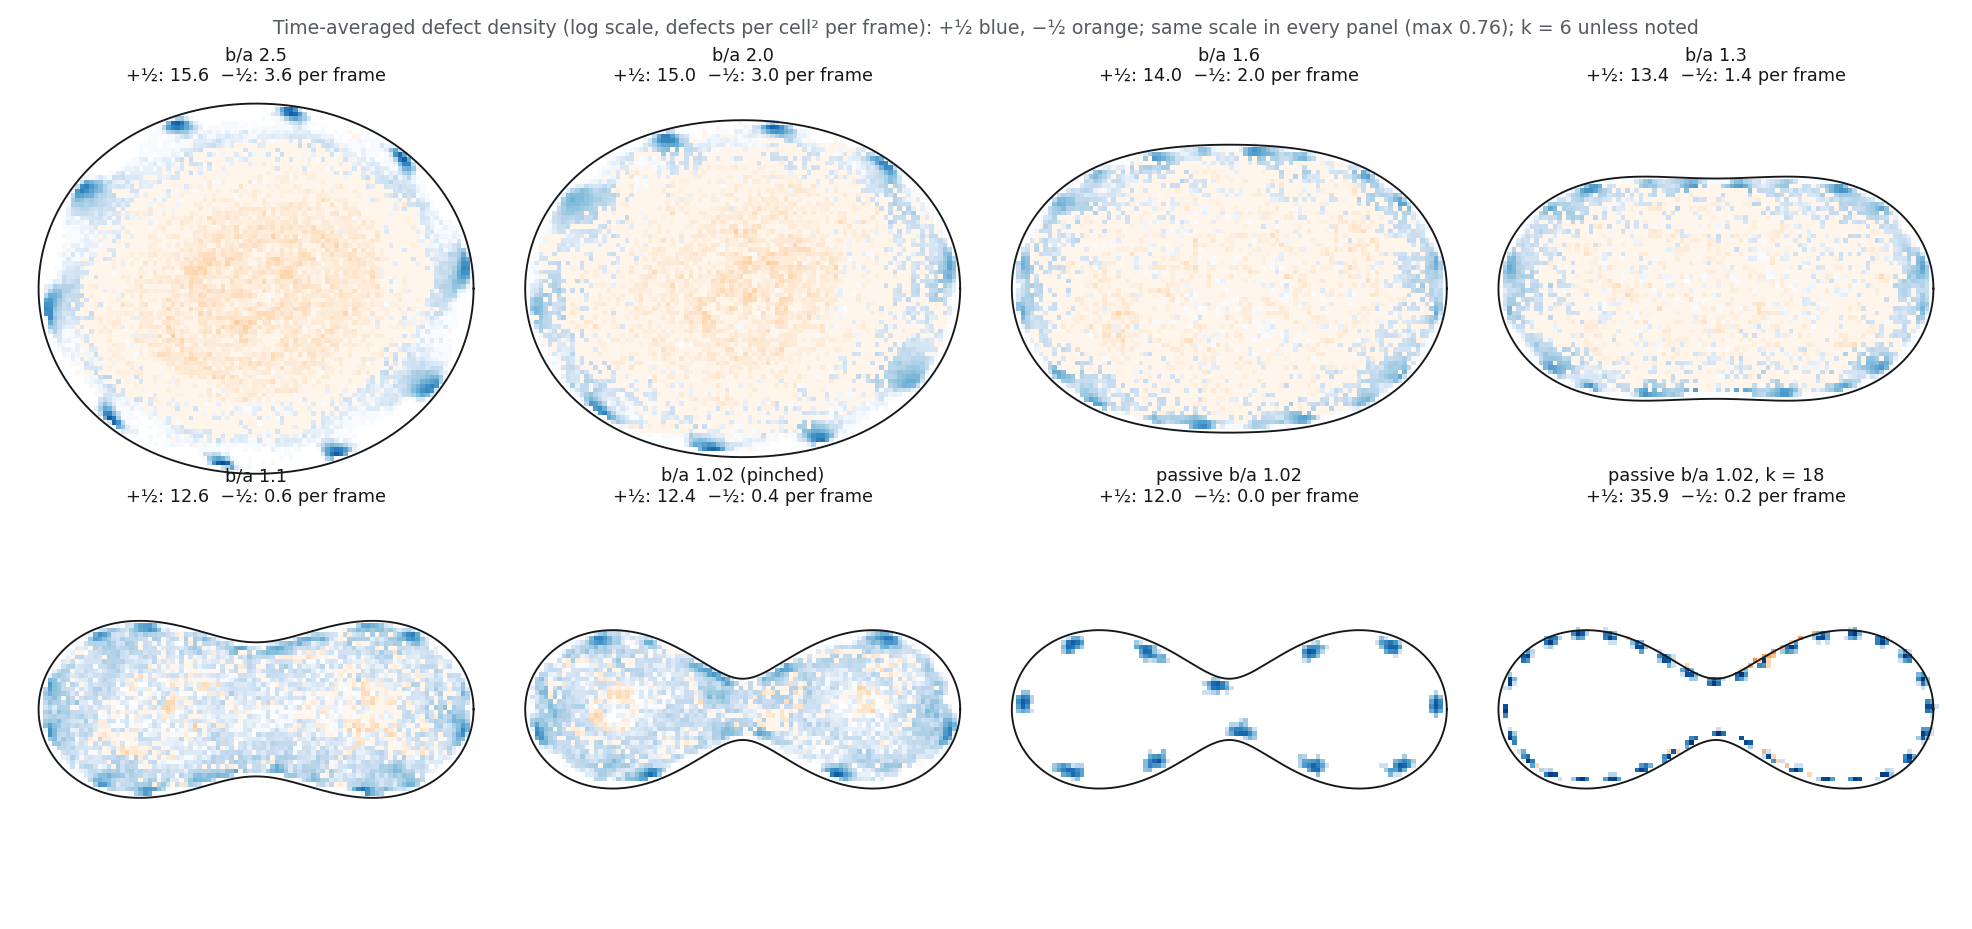
\includegraphics[width=\textwidth]{maps_ovals_large.png}
\caption{Ovals of half-length $2.16\,\la$, $k=6$: $b/a=2.5$, 2.0, 1.6, 1.3, 1.1 and the pinched 1.02 (active), the passive pinched
oval and the passive pinched oval at $k=18$.}\label{fig:maps-large}
\end{figure}
\begin{figure}[H]\centering
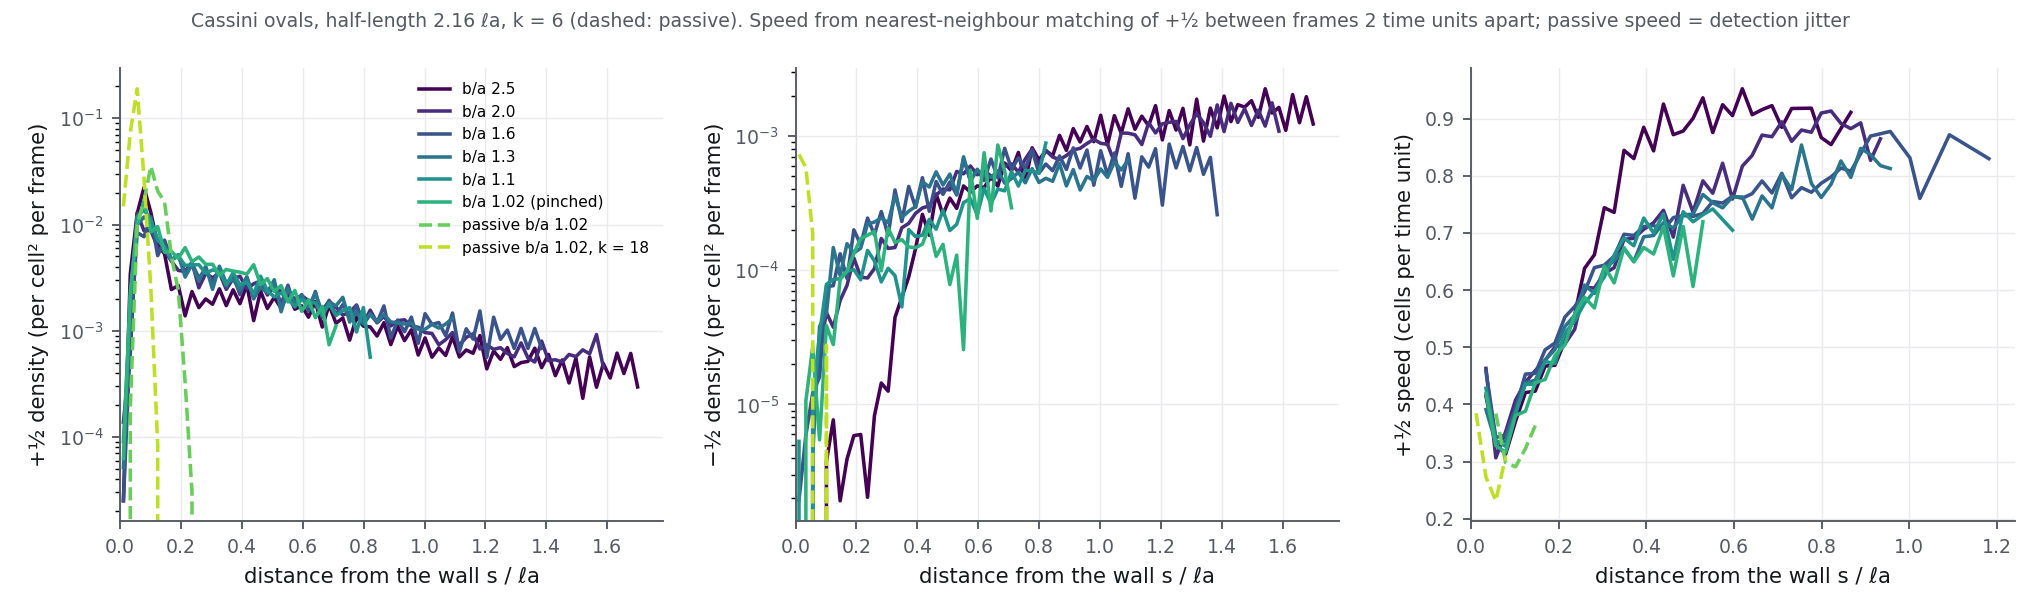
\includegraphics[width=\textwidth]{profiles_ovals_large.png}
\caption{Ovals of half-length $2.16\,\la$: profiles against the distance from the wall (dashed: passive).}\label{fig:prof-large}
\end{figure}
\begin{figure}[H]\centering
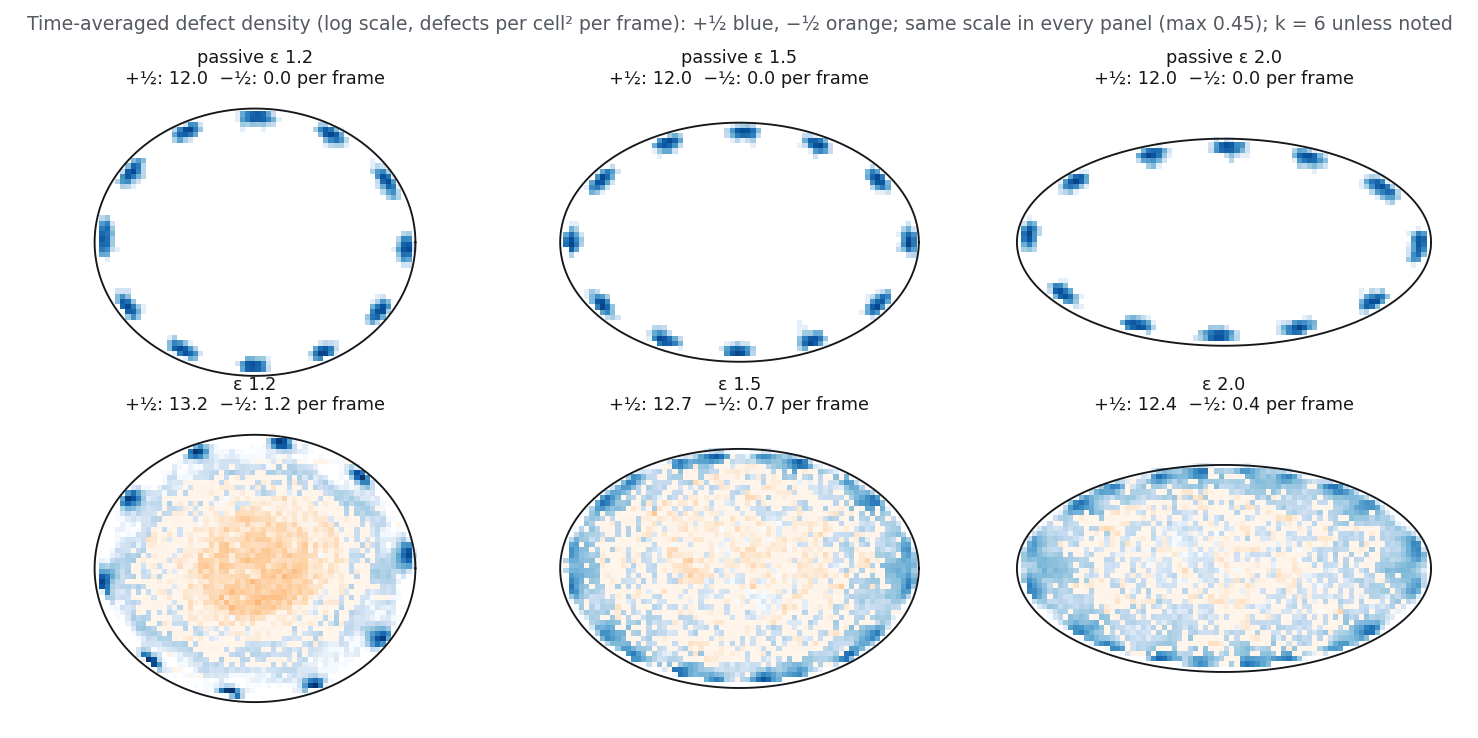
\includegraphics[width=0.92\textwidth]{maps_ellipses.png}
\caption{Ellipses (area 2500, $\sqrt{A/\pi}=1.27\,\la$), $k=6$: passive (top) and active (bottom), $\varepsilon=1.2$, 1.5, 2.0.}\label{fig:maps-ell}
\end{figure}
\begin{figure}[H]\centering
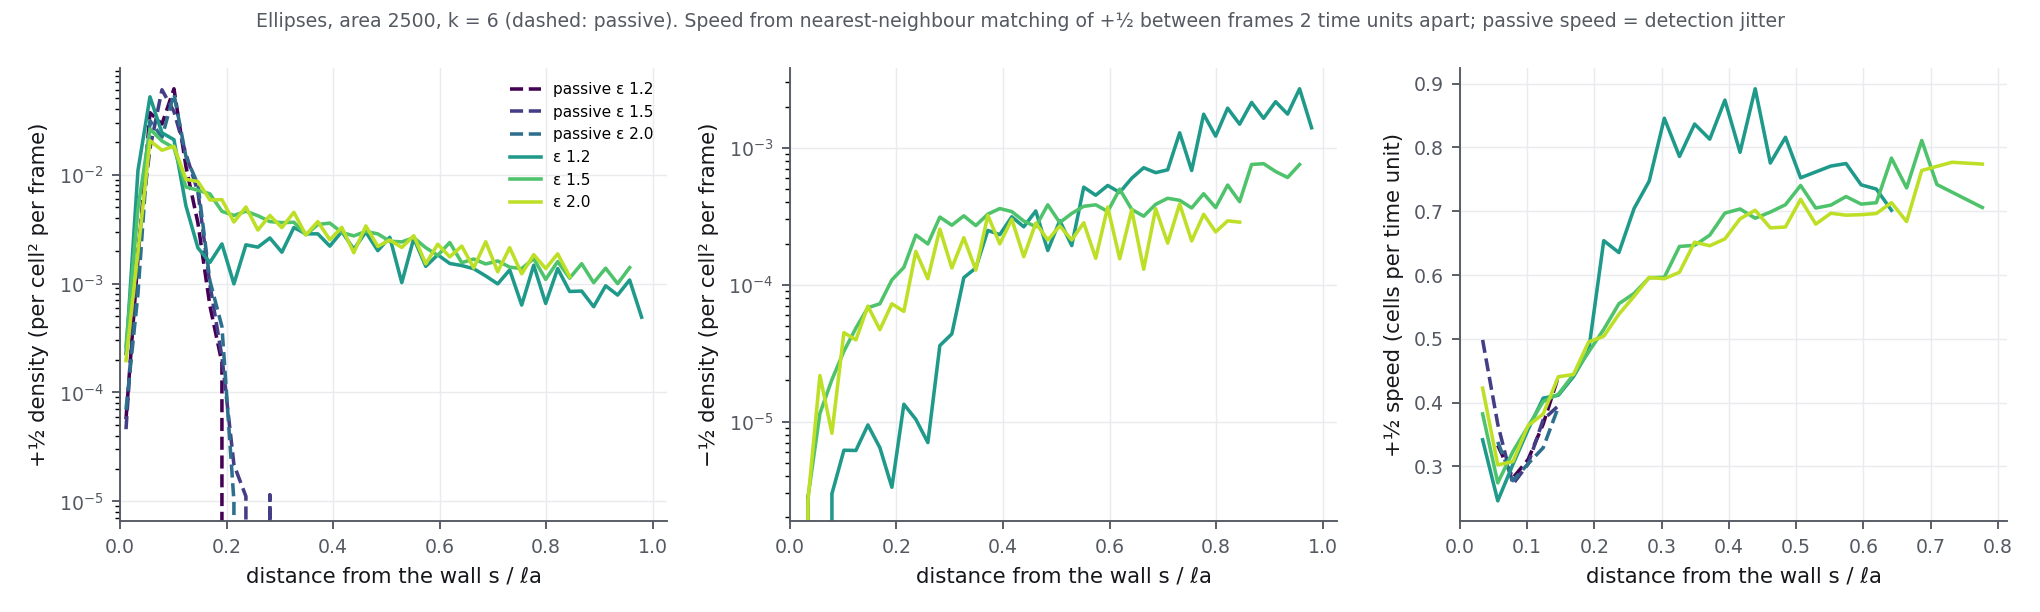
\includegraphics[width=\textwidth]{profiles_ellipses.png}
\caption{Ellipses: profiles against the distance from the wall (dashed: passive).}\label{fig:prof-ell}
\end{figure}
\begin{itemize}
  \item \textbf{Round shapes look like circles}: $b/a=2.5$ (aspect 1.17) and the ellipse $\varepsilon=1.2$ have 10 $=2k-2$ compact wall
        sites, a gap and a bulk with the $-\half$ in the centre.
  \item \textbf{Elongated shapes have no separate layer}: from aspect $\approx1.5$ the wall sites smear into a continuous band (at aspect 1.29 the sites are still discrete in these maps, but
        fewer are occupied; Secs.~\ref{sec:slattice}, \ref{sec:ssurv}),
        $+\half$ density rises steadily towards the wall without a gap, and far fewer $-\half$ are created (e.g.\ half-length
        $2.16\,\la$: 3.6 $-\half$ per frame at $b/a=2.5$, 2.0 at 1.6, 1.4 at 1.3, 0.4 in the pinched oval; the circle of the same
        half-length has 4.7). The $-\half$ no longer concentrate in one centre.
  \item In the pinched ovals defects accumulate at the neck, and each lobe has its own weak $-\half$ centre.
\end{itemize}
\begin{figure}[H]\centering
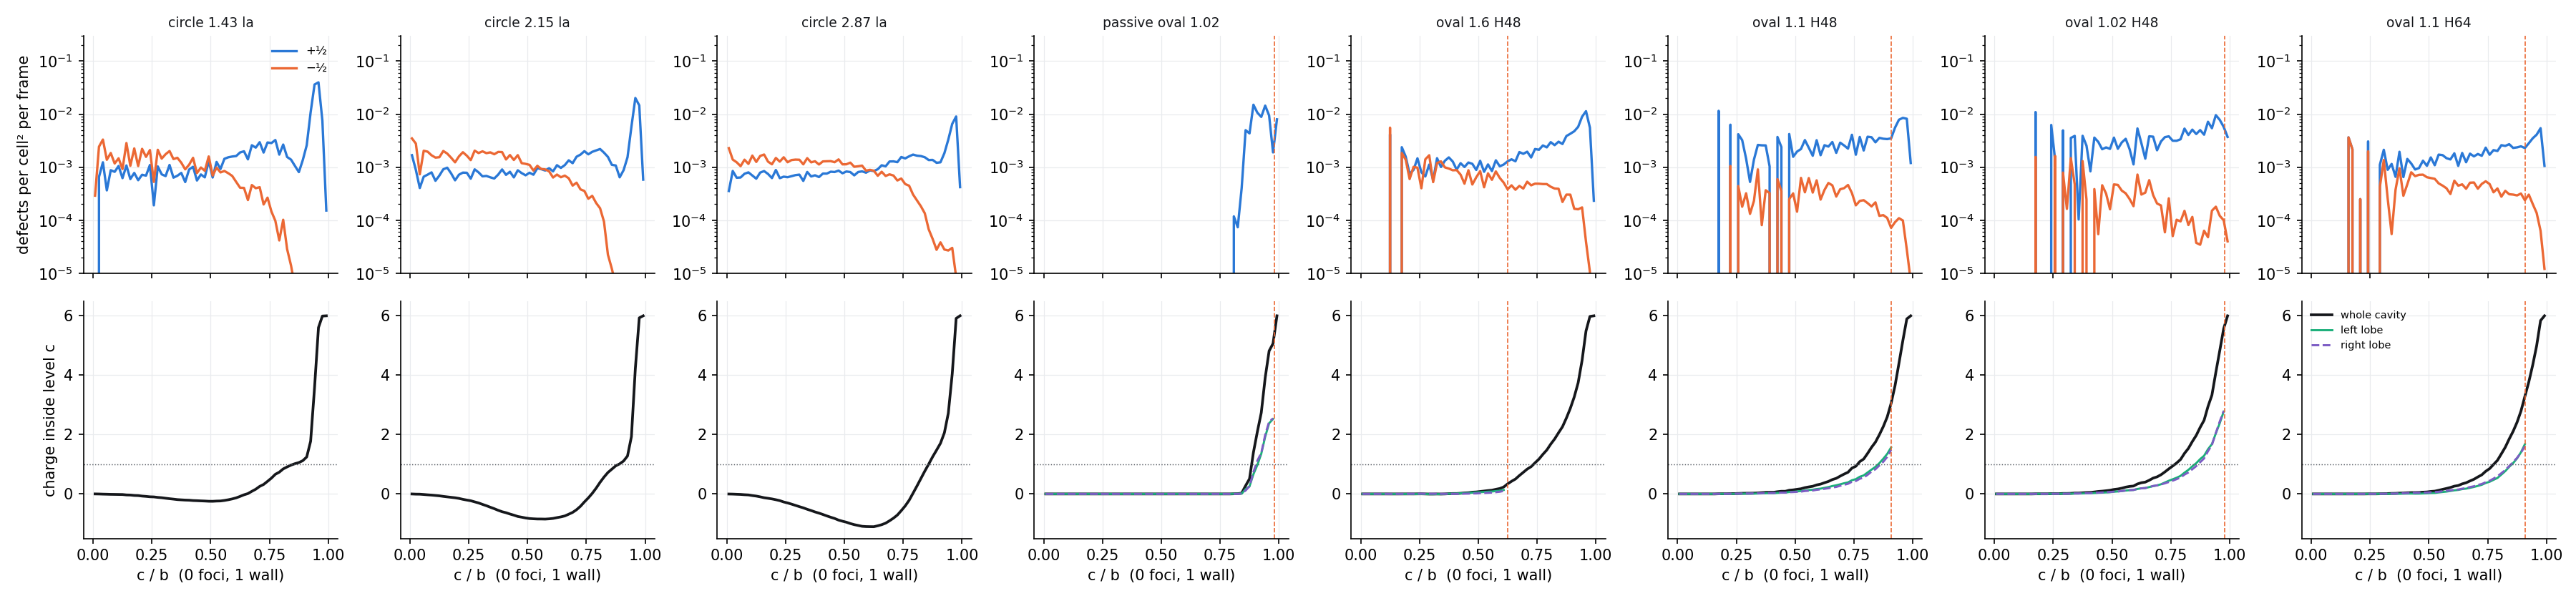
\includegraphics[width=\textwidth]{lobe_profiles_large.png}
\caption{Defect densities and accumulated charge in Cassini level coordinates $c=\sqrt{d_1d_2}$ (0 at the foci, $b$ at the wall)
for circles ($k=6$; 1.43, 2.15, $2.87\,\la$) and ovals of half-length 2.16 and $2.88\,\la$ (1 seed). Circles: $+\half$ wall peak at
$c/b\approx0.97$, dip inside it, negative $Q$ towards the centre. Ovals: $n_+$ rises steadily, no peak--gap structure.}\label{fig:lobeprof}
\end{figure}
\begin{figure}[H]\centering
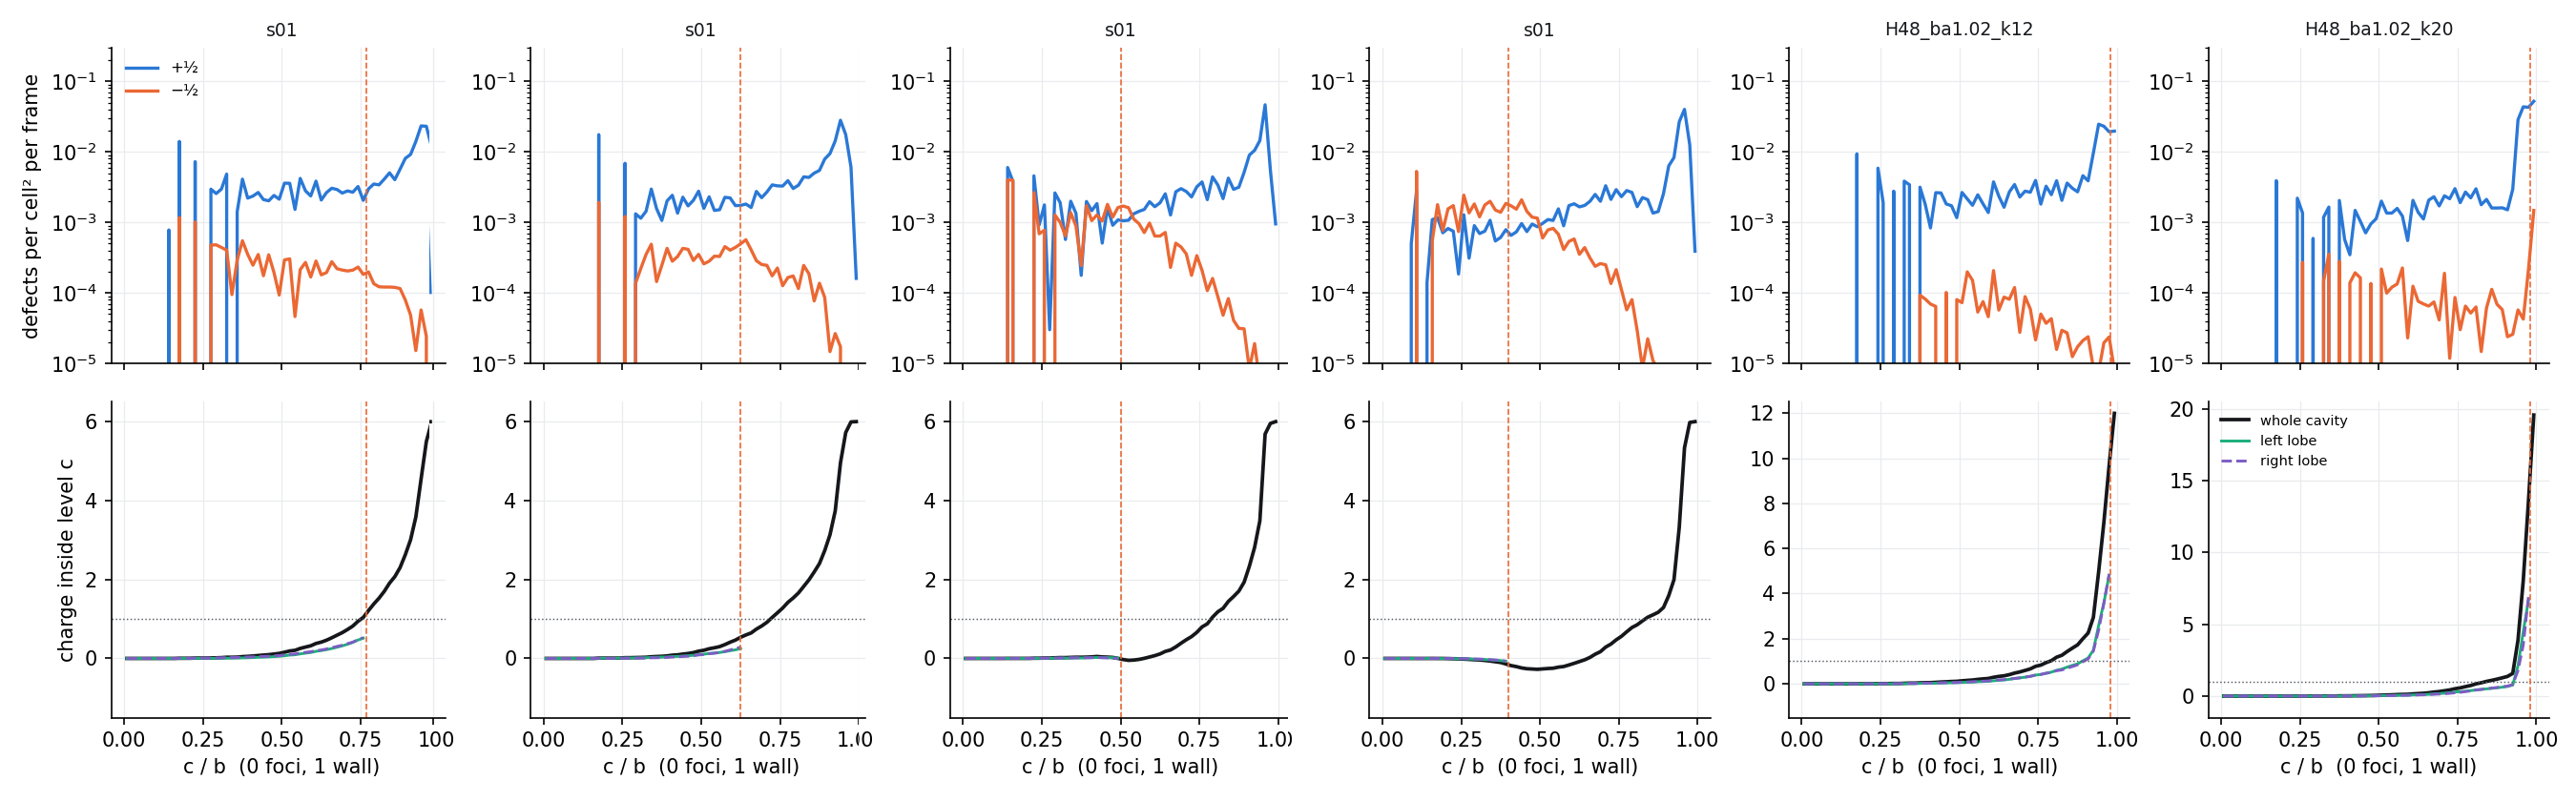
\includegraphics[width=\textwidth]{lobe_profiles_small_sel.png}
\caption{The same in level coordinates for seed 1 of the small ovals ($b/a=1.3$, 1.6, 2.0, 2.5; red line: lemniscate level $c=a$) and the pinched
oval at $k=12$, 20 (whole cavity and per-lobe $Q$). Top: $+\half$ (blue) and $-\half$ (orange) density; bottom: $Q(c)$.}\label{fig:lobeprof-small}
\end{figure}
\begin{figure}[H]\centering
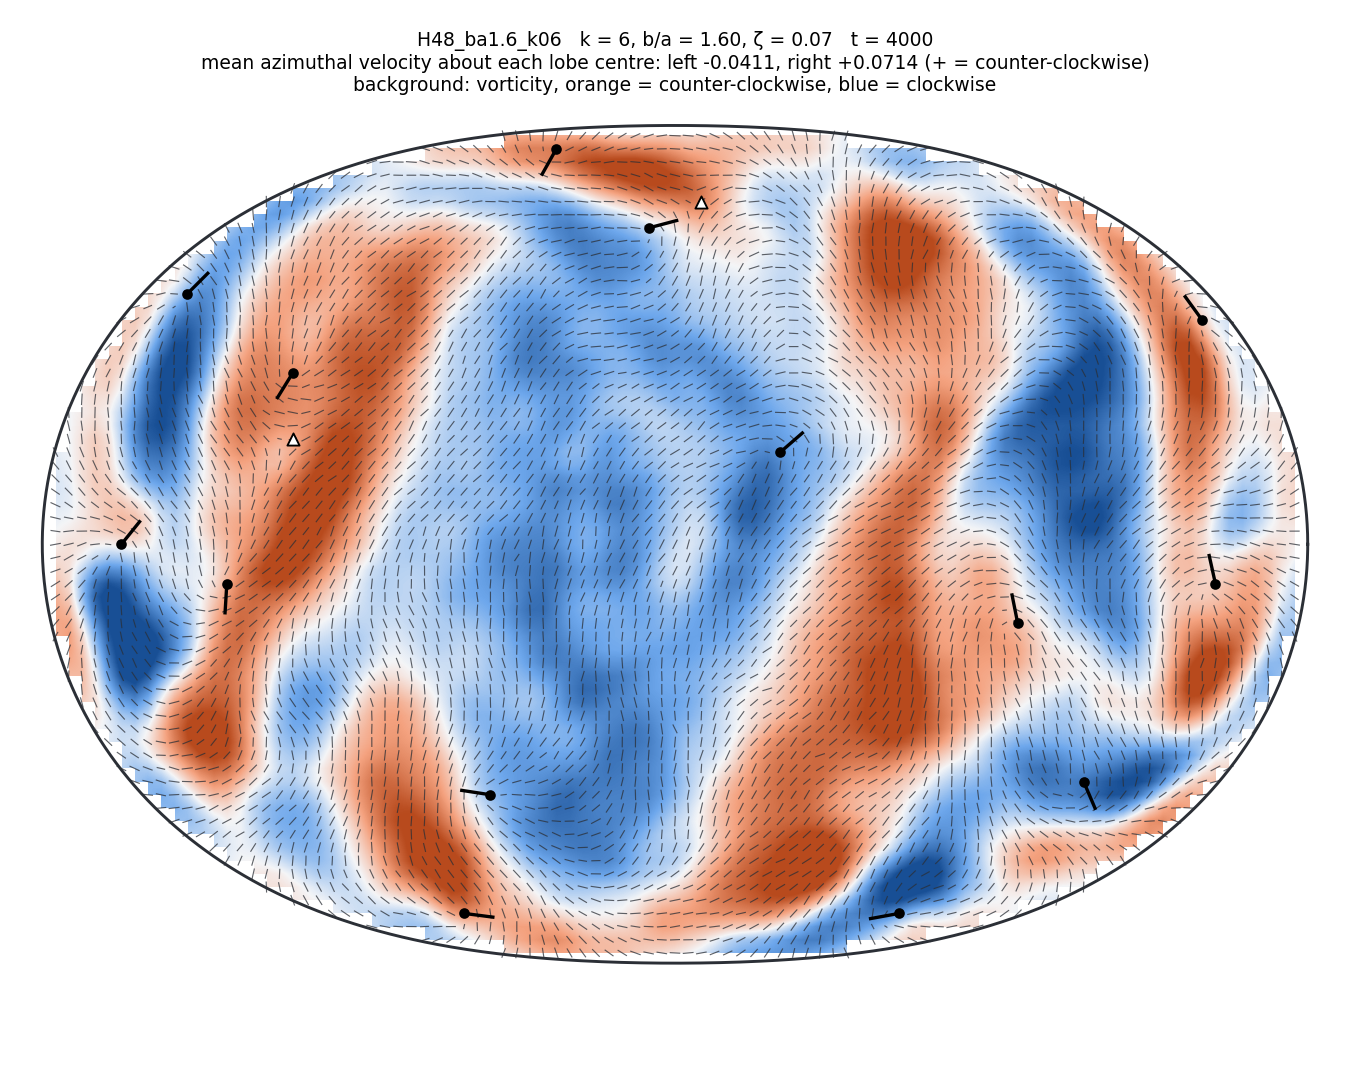
\includegraphics[width=0.49\textwidth]{snap_ba1.6.png}\hfill
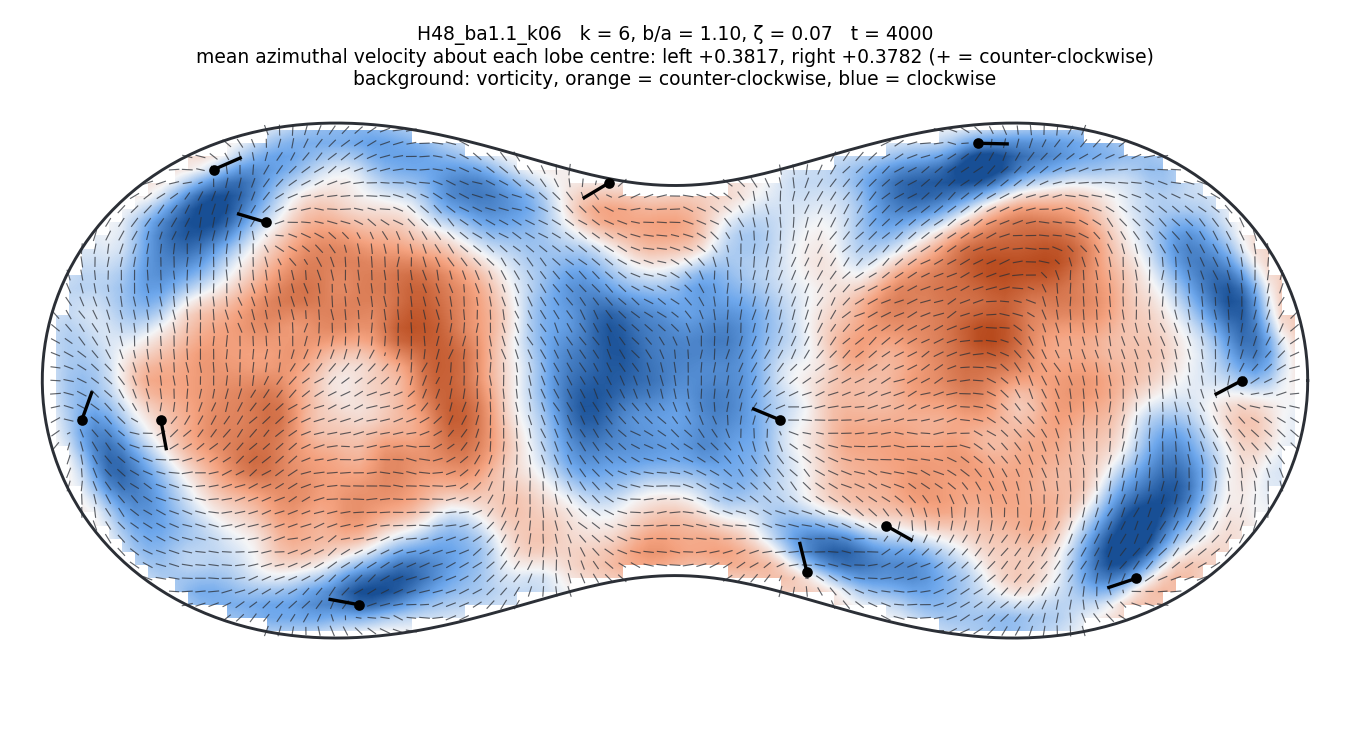
\includegraphics[width=0.49\textwidth]{snap_ba1.1.png}\\[4pt]
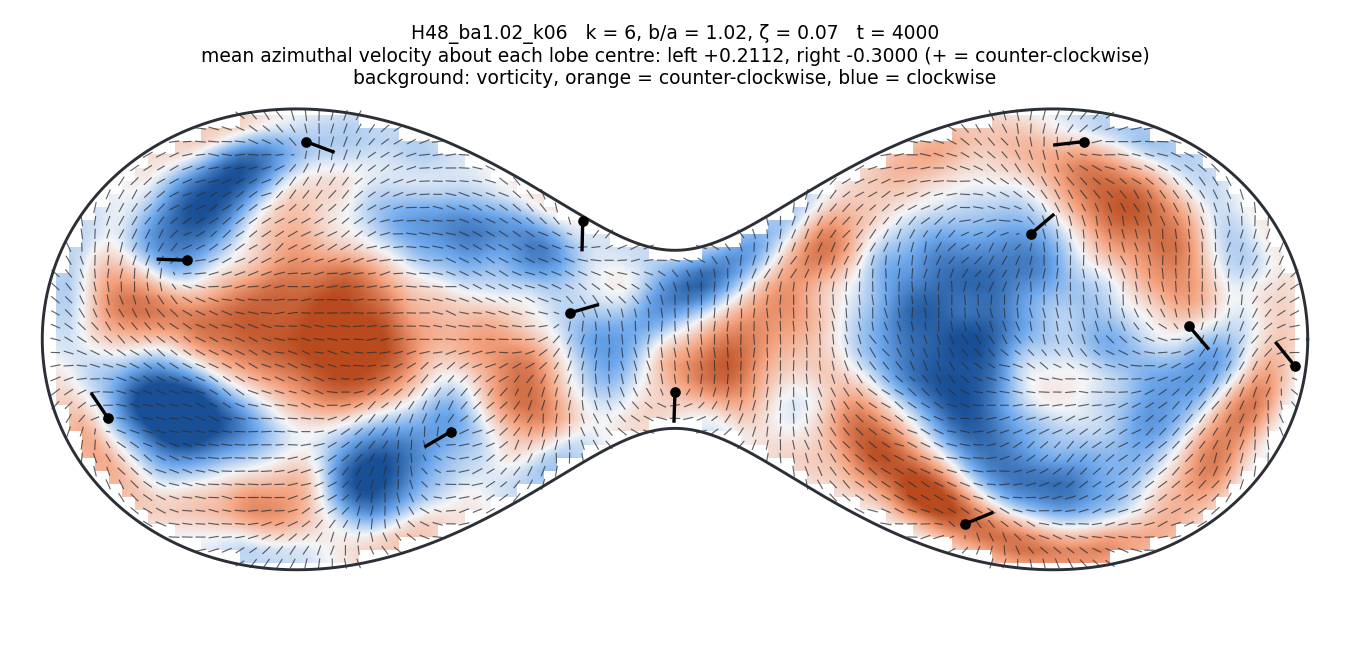
\includegraphics[width=0.49\textwidth]{snap_ba1.02.png}\hfill
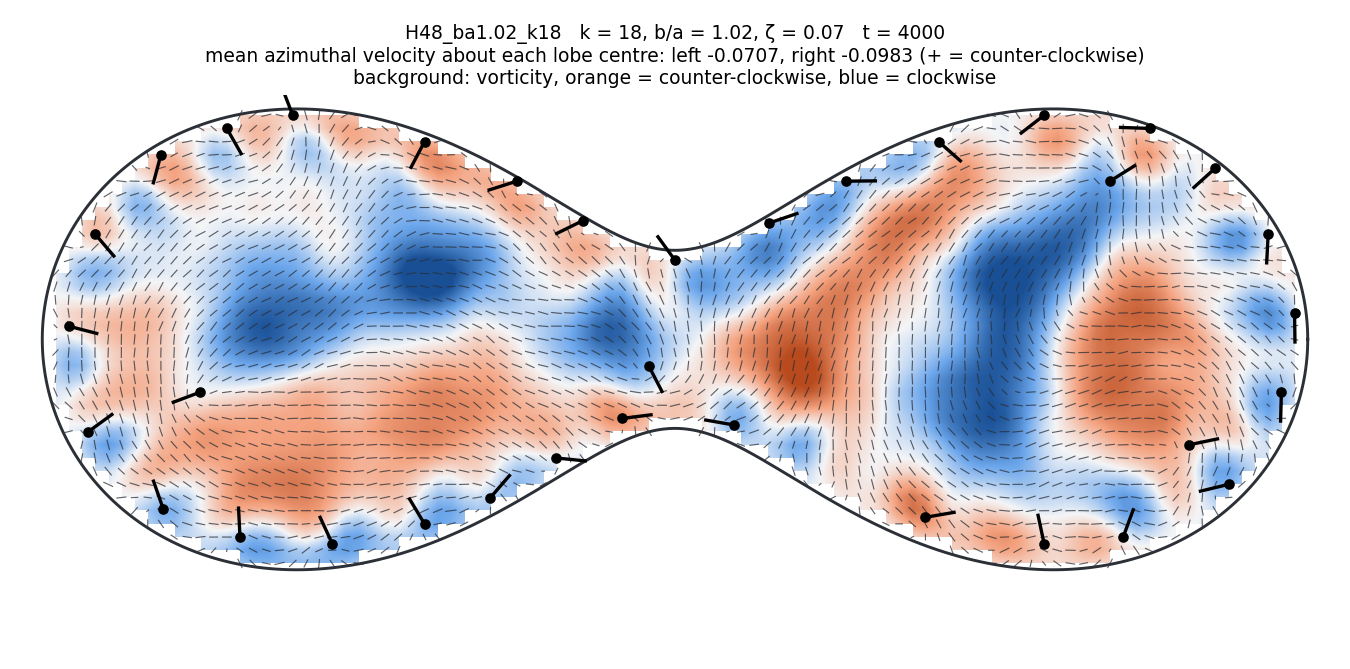
\includegraphics[width=0.49\textwidth]{snap_ba1.02_k18.png}
\caption{Snapshots at the end of the runs (half-length $2.16\,\la$): vorticity (orange counter-clockwise, blue clockwise), director,
$+\half$ (dots with orientation tail), $-\half$ (triangles). $b/a=1.6$, 1.1, 1.02 ($k=6$) and 1.02 at $k=18$. Movies:
\texttt{results/6\_shape/movies/}.}\label{fig:snaps}
\end{figure}
